\documentclass[10pt,a4paper]{article}
\usepackage[utf8]{inputenc}
\usepackage[T1]{fontenc}
\usepackage{amsmath}
\usepackage{amsfonts}
\usepackage{amssymb}
\usepackage{natbib}
\usepackage{graphicx}

\title{Maths theory}
\author{Max Cotton}
\date{}

\begin{document}

\maketitle

\section{Dot Product}

\begin{figure}[h!]
\centering
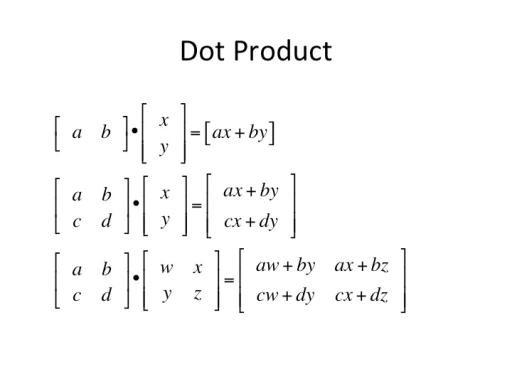
\includegraphics[width=0.8\textwidth]{./docs/models/src/images/dot-product.png}
\end{figure}

Note that the order the matrices are multiplied in is important

\begin{itemize}
    \item The "Dot Product" multiplies the row of one matrice with the column of the other, by multiplying matching members and then summing up. 
    \item The number of columns of the 1st matrix must equal the number of rows of the 2nd matrix. And the result will have the same number of rows as the 1st matrix, and the same number of columns as the 2nd matrix.
\end{itemize}

\section{Partial Derivatives}

\begin{itemize}
    \item The "Partial Derivative" is the derivative of a function with more than one variable, by having respect to only one variable and treating the other/s as a constant
\end{itemize}

\section{Chain Rule of Differentiation}

\begin{figure}[h!]
\centering
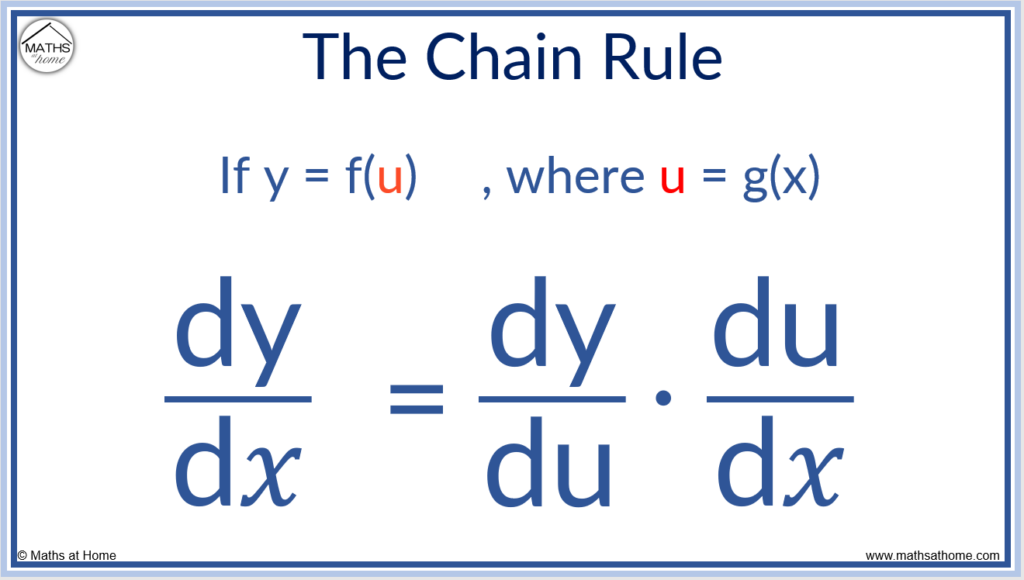
\includegraphics[width=0.5\textwidth]{./docs/models/src/images/chain-rule.png}
\end{figure}

Note that $\frac{\partial{y}}{\partial{x}}$, means derivative of y with respect to x

\end{document}